\begin{figure}
  \centering 
  \begin{subfigure}[b]{0.45\textwidth}
    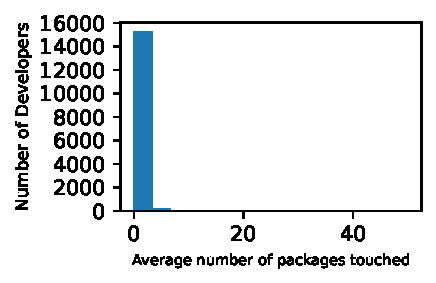
\includegraphics[width=\textwidth]{sections/results/graph/normality_and_homoscedasticity_graph_transient_moderate_1_packages_founder_transient.packages.touched.commits.pdf}
    \caption{Transient ($\mu$: 1.15, median:1.0, mode:1, std:0.92 and max:50)}
    \label{figure.sections/results/graph/normality_and_homoscedasticity_graph_transient_moderate_1_packages_founder_transient.packages.touched.commits.pdf}
  \end{subfigure}
  \begin{subfigure}[b]{0.45\textwidth}
    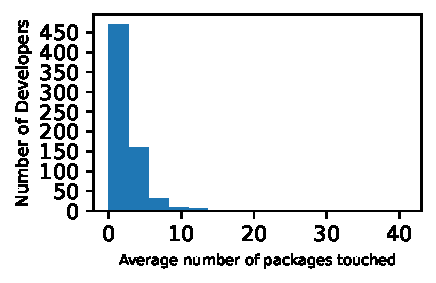
\includegraphics[width=\textwidth]{sections/results/graph/normality_and_homoscedasticity_graph_transient_moderate_1_packages_sample_moderate.packages.touched.commits.pdf}
    \caption{Moderate ($\mu$: 2.59, median:2, mode:1, std:3.06 and max:41)}
    \label{figure.sections/results/graph/normality_and_homoscedasticity_graph_transient_moderate_1_packages_sample_moderate.packages.touched.commits.pdf}
  \end{subfigure}
\vspace{3mm}
  \begin{subfigure}[b]{0.45\textwidth}
    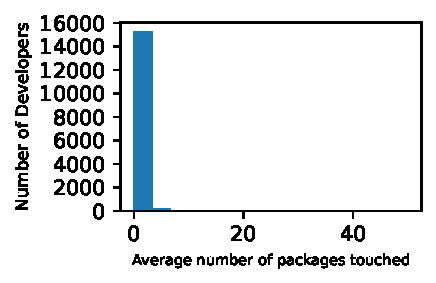
\includegraphics[width=\textwidth]{sections/results/graph/normality_and_homoscedasticity_graph_transient_moderate_1_packages_founder_transient.packages.touched.commits.pdf}
    \caption{Transient ($\mu$: 1.15, median:1.0, mode:1, std:0.92 and max:50)}
    \label{figure.sections/results/graph/normality_and_homoscedasticity_graph_transient_moderate_1_packages_founder_transient.packages.touched.commits.pdf}
  \end{subfigure}
  \begin{subfigure}[b]{0.45\textwidth}
    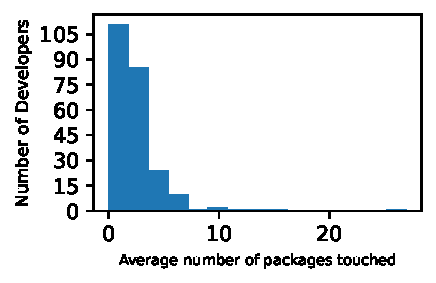
\includegraphics[width=\textwidth]{sections/results/graph/normality_and_homoscedasticity_graph_transient_moderate_1_packages_sample_sustained.packages.touched.commits.pdf}
    \caption{Sustained ($\mu$: 2.38, median:2, mode:1, std:2.61 and max:27)}
    \label{figure.sections/results/graph/normality_and_homoscedasticity_graph_transient_moderate_1_packages_sample_sustained.packages.touched.commits.pdf}
  \end{subfigure}
\vspace{3mm}
  \begin{subfigure}[b]{0.45\textwidth}
    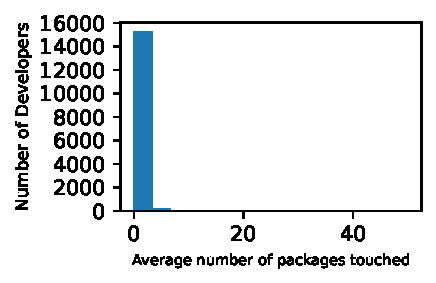
\includegraphics[width=\textwidth]{sections/results/graph/normality_and_homoscedasticity_graph_transient_moderate_1_packages_founder_transient.packages.touched.commits.pdf}
    \caption{Transient ($\mu$: 1.15, median:1.0, mode:1, std:0.92 and max:50)}
    \label{figure.sections/results/graph/normality_and_homoscedasticity_graph_transient_moderate_1_packages_founder_transient.packages.touched.commits.pdf}
  \end{subfigure}
  \begin{subfigure}[b]{0.45\textwidth}
    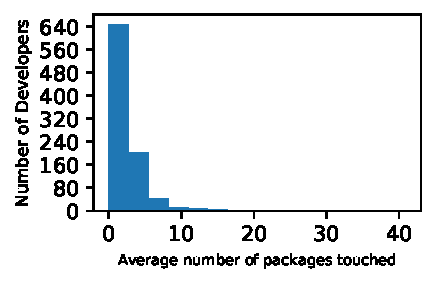
\includegraphics[width=\textwidth]{sections/results/graph/normality_and_homoscedasticity_graph_transient_moderate_1_packages_sample_moderate sustained.packages.touched.commits.pdf}
    \caption{Moderate sustained ($\mu$: 2.54, median:2.0, mode:1, std:2.95 and max:41)}
    \label{figure.sections/results/graph/normality_and_homoscedasticity_graph_transient_moderate_1_packages_sample_moderate sustained.packages.touched.commits.pdf}
  \end{subfigure}
\vspace{3mm}
  \begin{subfigure}[b]{0.45\textwidth}
    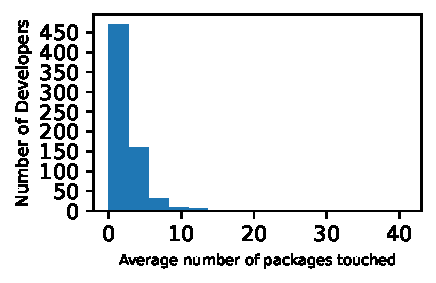
\includegraphics[width=\textwidth]{sections/results/graph/normality_and_homoscedasticity_graph_transient_moderate_1_packages_founder_moderate.packages.touched.commits.pdf}
    \caption{Moderate ($\mu$: 2.59, median:2, mode:1, std:3.06 and max:41)}
    \label{figure.sections/results/graph/normality_and_homoscedasticity_graph_transient_moderate_1_packages_founder_moderate.packages.touched.commits.pdf}
  \end{subfigure}
  \begin{subfigure}[b]{0.45\textwidth}
    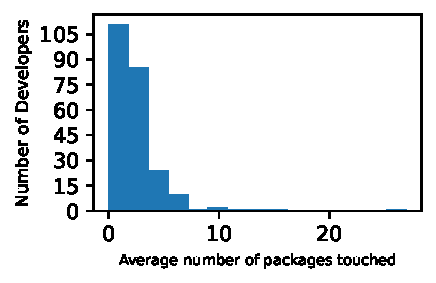
\includegraphics[width=\textwidth]{sections/results/graph/normality_and_homoscedasticity_graph_transient_moderate_1_packages_sample_sustained.packages.touched.commits.pdf}
    \caption{Sustained ($\mu$: 2.38, median:2, mode:1, std:2.61 and max:27)}
    \label{figure.sections/results/graph/normality_and_homoscedasticity_graph_transient_moderate_1_packages_sample_sustained.packages.touched.commits.pdf}
  \end{subfigure}
\caption{Packages for one commits for  sample A category versus sample B category } 
\end{figure}
\clearpage 
\begin{figure}
  \centering 
\vspace{3mm}
  \begin{subfigure}[b]{0.45\textwidth}
    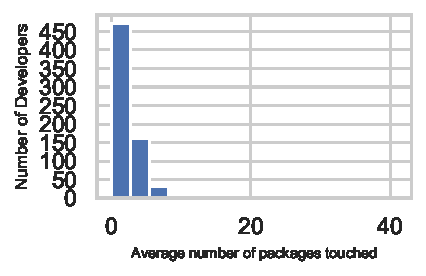
\includegraphics[width=\textwidth]{sections/results/graph/normality_and_homoscedasticity_graph_transient_moderate_2_packages_founder_moderate.packages.touched.commits.pdf}
    \caption{Moderate ($\mu$: 3.58, median:3, mode:2, std:3.82 and max:46)}
    \label{figure.sections/results/graph/normality_and_homoscedasticity_graph_transient_moderate_2_packages_founder_moderate.packages.touched.commits.pdf}
  \end{subfigure}
  \begin{subfigure}[b]{0.45\textwidth}
    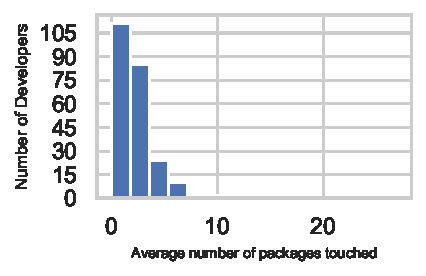
\includegraphics[width=\textwidth]{sections/results/graph/normality_and_homoscedasticity_graph_transient_moderate_2_packages_sample_sustained.packages.touched.commits.pdf}
    \caption{Sustained ($\mu$: 3.49, median:2, mode:2, std:4.51 and max:55)}
    \label{figure.sections/results/graph/normality_and_homoscedasticity_graph_transient_moderate_2_packages_sample_sustained.packages.touched.commits.pdf}
  \end{subfigure}
\caption{Packages for two commits for  sample A category versus sample B category } 
\end{figure}
\clearpage 
\begin{figure}
  \centering 
\vspace{3mm}
  \begin{subfigure}[b]{0.45\textwidth}
    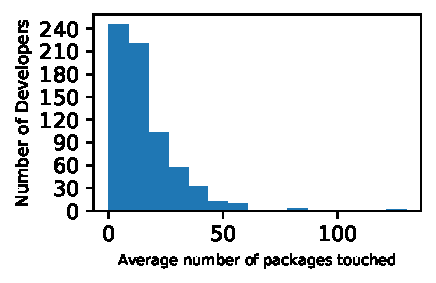
\includegraphics[width=\textwidth]{sections/results/graph/normality_and_homoscedasticity_graph_transient_moderate_5_packages_founder_moderate.packages.touched.commits.pdf}
    \caption{Moderate ($\mu$: 6.34, median:5, mode:4, std:5.65 and max:47)}
    \label{figure.sections/results/graph/normality_and_homoscedasticity_graph_transient_moderate_5_packages_founder_moderate.packages.touched.commits.pdf}
  \end{subfigure}
  \begin{subfigure}[b]{0.45\textwidth}
    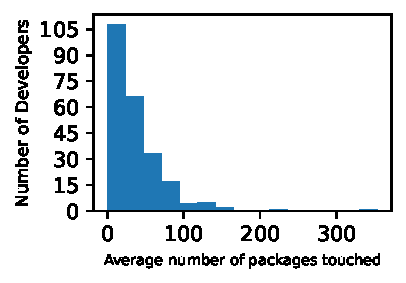
\includegraphics[width=\textwidth]{sections/results/graph/normality_and_homoscedasticity_graph_transient_moderate_5_packages_sample_sustained.packages.touched.commits.pdf}
    \caption{Sustained ($\mu$: 5.93, median:4, mode:3, std:5.99 and max:58)}
    \label{figure.sections/results/graph/normality_and_homoscedasticity_graph_transient_moderate_5_packages_sample_sustained.packages.touched.commits.pdf}
  \end{subfigure}
\caption{Packages for five commits for  sample A category versus sample B category } 
\end{figure}
\clearpage 
\begin{figure}
  \centering 
\vspace{3mm}
  \begin{subfigure}[b]{0.45\textwidth}
    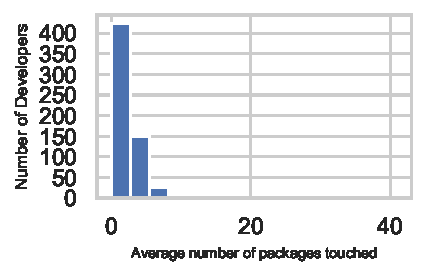
\includegraphics[width=\textwidth]{sections/results/graph/normality_and_homoscedasticity_graph_transient_moderate_10_packages_founder_moderate.packages.touched.commits.pdf}
    \caption{Moderate ($\mu$: 9.62, median:8.0, mode:6, std:7.33 and max:50)}
    \label{figure.sections/results/graph/normality_and_homoscedasticity_graph_transient_moderate_10_packages_founder_moderate.packages.touched.commits.pdf}
  \end{subfigure}
  \begin{subfigure}[b]{0.45\textwidth}
    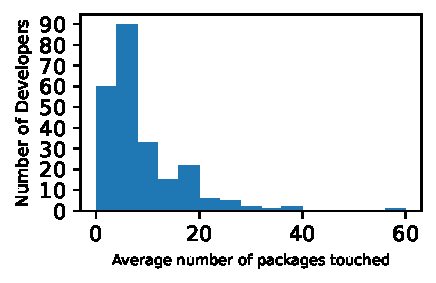
\includegraphics[width=\textwidth]{sections/results/graph/normality_and_homoscedasticity_graph_transient_moderate_10_packages_sample_sustained.packages.touched.commits.pdf}
    \caption{Sustained ($\mu$: 8.36, median:6, mode:5, std:7.67 and max:60)}
    \label{figure.sections/results/graph/normality_and_homoscedasticity_graph_transient_moderate_10_packages_sample_sustained.packages.touched.commits.pdf}
  \end{subfigure}
\caption{Packages for ten commits for  sample A category versus sample B category } 
\end{figure}
\clearpage 
\begin{figure}
  \centering 
\end{figure}
\clearpage 
\begin{figure}
  \centering 
\vspace{3mm}
  \begin{subfigure}[b]{0.45\textwidth}
    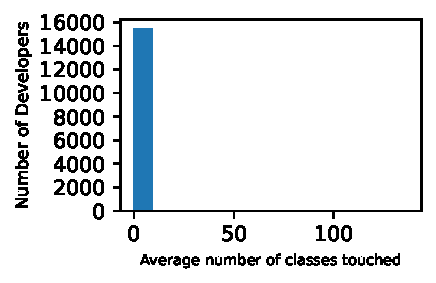
\includegraphics[width=\textwidth]{sections/results/graph/normality_and_homoscedasticity_graph_transient_moderate_1_classes_founder_transient.classes.touched.commits.pdf}
    \caption{Transient ($\mu$: 1.15, median:1.0, mode:1, std:1.95 and max:137)}
    \label{figure.sections/results/graph/normality_and_homoscedasticity_graph_transient_moderate_1_classes_founder_transient.classes.touched.commits.pdf}
  \end{subfigure}
  \begin{subfigure}[b]{0.45\textwidth}
    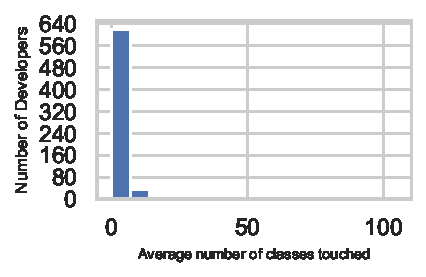
\includegraphics[width=\textwidth]{sections/results/graph/normality_and_homoscedasticity_graph_transient_moderate_1_classes_sample_moderate.classes.touched.commits.pdf}
    \caption{Moderate ($\mu$: 3.24, median:1, mode:1, std:8.5 and max:105)}
    \label{figure.sections/results/graph/normality_and_homoscedasticity_graph_transient_moderate_1_classes_sample_moderate.classes.touched.commits.pdf}
  \end{subfigure}
\vspace{3mm}
  \begin{subfigure}[b]{0.45\textwidth}
    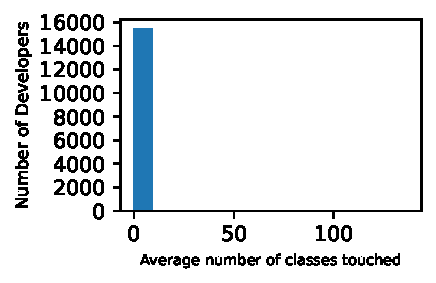
\includegraphics[width=\textwidth]{sections/results/graph/normality_and_homoscedasticity_graph_transient_moderate_1_classes_founder_transient.classes.touched.commits.pdf}
    \caption{Transient ($\mu$: 1.15, median:1.0, mode:1, std:1.95 and max:137)}
    \label{figure.sections/results/graph/normality_and_homoscedasticity_graph_transient_moderate_1_classes_founder_transient.classes.touched.commits.pdf}
  \end{subfigure}
  \begin{subfigure}[b]{0.45\textwidth}
    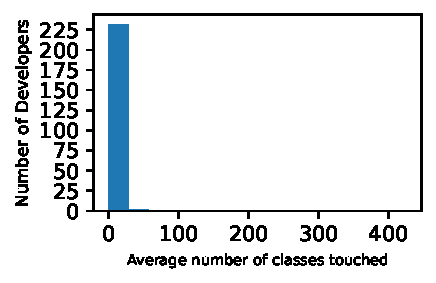
\includegraphics[width=\textwidth]{sections/results/graph/normality_and_homoscedasticity_graph_transient_moderate_1_classes_sample_sustained.classes.touched.commits.pdf}
    \caption{Sustained ($\mu$: 5.19, median:1, mode:1, std:30.1 and max:426)}
    \label{figure.sections/results/graph/normality_and_homoscedasticity_graph_transient_moderate_1_classes_sample_sustained.classes.touched.commits.pdf}
  \end{subfigure}
\vspace{3mm}
  \begin{subfigure}[b]{0.45\textwidth}
    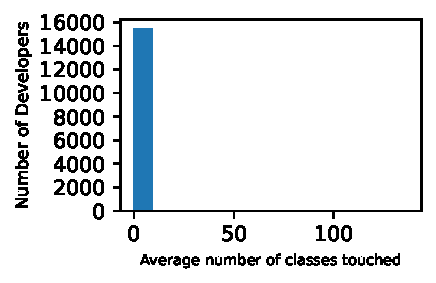
\includegraphics[width=\textwidth]{sections/results/graph/normality_and_homoscedasticity_graph_transient_moderate_1_classes_founder_transient.classes.touched.commits.pdf}
    \caption{Transient ($\mu$: 1.15, median:1.0, mode:1, std:1.95 and max:137)}
    \label{figure.sections/results/graph/normality_and_homoscedasticity_graph_transient_moderate_1_classes_founder_transient.classes.touched.commits.pdf}
  \end{subfigure}
  \begin{subfigure}[b]{0.45\textwidth}
    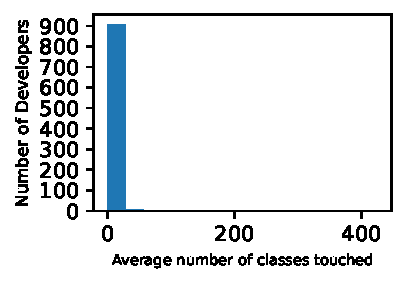
\includegraphics[width=\textwidth]{sections/results/graph/normality_and_homoscedasticity_graph_transient_moderate_1_classes_sample_moderate sustained.classes.touched.commits.pdf}
    \caption{Moderate sustained ($\mu$: 3.74, median:1.0, mode:1, std:16.92 and max:426)}
    \label{figure.sections/results/graph/normality_and_homoscedasticity_graph_transient_moderate_1_classes_sample_moderate sustained.classes.touched.commits.pdf}
  \end{subfigure}
\vspace{3mm}
  \begin{subfigure}[b]{0.45\textwidth}
    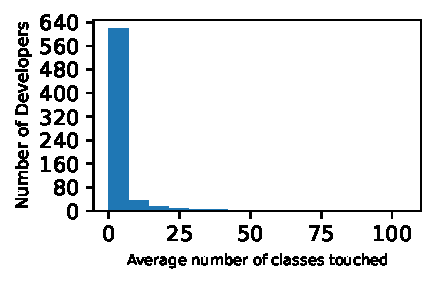
\includegraphics[width=\textwidth]{sections/results/graph/normality_and_homoscedasticity_graph_transient_moderate_1_classes_founder_moderate.classes.touched.commits.pdf}
    \caption{Moderate ($\mu$: 3.24, median:1, mode:1, std:8.5 and max:105)}
    \label{figure.sections/results/graph/normality_and_homoscedasticity_graph_transient_moderate_1_classes_founder_moderate.classes.touched.commits.pdf}
  \end{subfigure}
  \begin{subfigure}[b]{0.45\textwidth}
    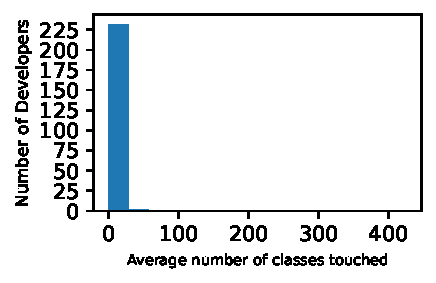
\includegraphics[width=\textwidth]{sections/results/graph/normality_and_homoscedasticity_graph_transient_moderate_1_classes_sample_sustained.classes.touched.commits.pdf}
    \caption{Sustained ($\mu$: 5.19, median:1, mode:1, std:30.1 and max:426)}
    \label{figure.sections/results/graph/normality_and_homoscedasticity_graph_transient_moderate_1_classes_sample_sustained.classes.touched.commits.pdf}
  \end{subfigure}
\caption{Classes for one commits for  sample A category versus sample B category } 
\end{figure}
\clearpage 
\begin{figure}
  \centering 
\vspace{3mm}
  \begin{subfigure}[b]{0.45\textwidth}
    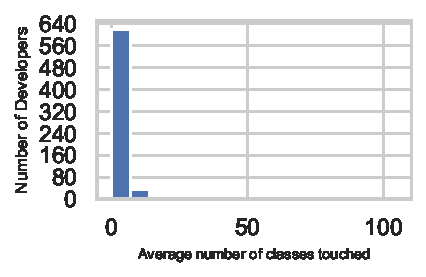
\includegraphics[width=\textwidth]{sections/results/graph/normality_and_homoscedasticity_graph_transient_moderate_2_classes_founder_moderate.classes.touched.commits.pdf}
    \caption{Moderate ($\mu$: 8.48, median:3, mode:1, std:17.02 and max:174)}
    \label{figure.sections/results/graph/normality_and_homoscedasticity_graph_transient_moderate_2_classes_founder_moderate.classes.touched.commits.pdf}
  \end{subfigure}
  \begin{subfigure}[b]{0.45\textwidth}
    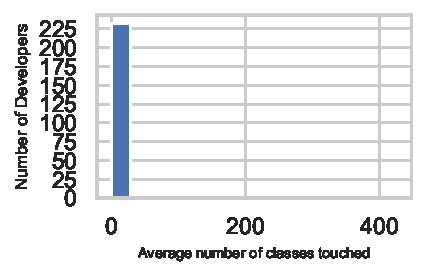
\includegraphics[width=\textwidth]{sections/results/graph/normality_and_homoscedasticity_graph_transient_moderate_2_classes_sample_sustained.classes.touched.commits.pdf}
    \caption{Sustained ($\mu$: 9.88, median:3, mode:1, std:37.38 and max:386)}
    \label{figure.sections/results/graph/normality_and_homoscedasticity_graph_transient_moderate_2_classes_sample_sustained.classes.touched.commits.pdf}
  \end{subfigure}
\caption{Classes for two commits for  sample A category versus sample B category } 
\end{figure}
\clearpage 
\begin{figure}
  \centering 
\vspace{3mm}
  \begin{subfigure}[b]{0.45\textwidth}
    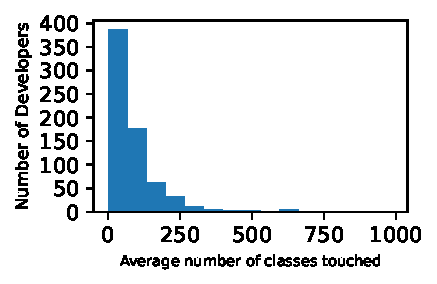
\includegraphics[width=\textwidth]{sections/results/graph/normality_and_homoscedasticity_graph_transient_moderate_5_classes_founder_moderate.classes.touched.commits.pdf}
    \caption{Moderate ($\mu$: 24.02, median:15, mode:6, std:32.67 and max:442)}
    \label{figure.sections/results/graph/normality_and_homoscedasticity_graph_transient_moderate_5_classes_founder_moderate.classes.touched.commits.pdf}
  \end{subfigure}
  \begin{subfigure}[b]{0.45\textwidth}
    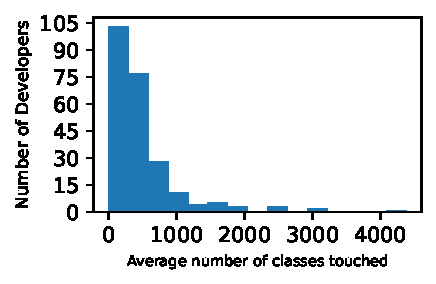
\includegraphics[width=\textwidth]{sections/results/graph/normality_and_homoscedasticity_graph_transient_moderate_5_classes_sample_sustained.classes.touched.commits.pdf}
    \caption{Sustained ($\mu$: 30.92, median:14, mode:9, std:66.72 and max:582)}
    \label{figure.sections/results/graph/normality_and_homoscedasticity_graph_transient_moderate_5_classes_sample_sustained.classes.touched.commits.pdf}
  \end{subfigure}
\caption{Classes for five commits for  sample A category versus sample B category } 
\end{figure}
\clearpage 
\begin{figure}
  \centering 
\vspace{3mm}
  \begin{subfigure}[b]{0.45\textwidth}
    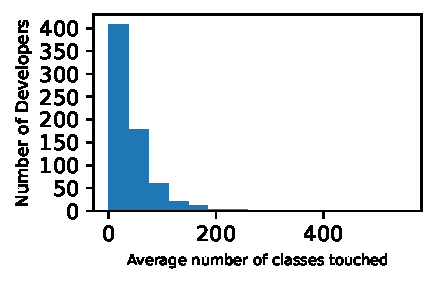
\includegraphics[width=\textwidth]{sections/results/graph/normality_and_homoscedasticity_graph_transient_moderate_10_classes_founder_moderate.classes.touched.commits.pdf}
    \caption{Moderate ($\mu$: 43.22, median:31.0, mode:28, std:44.05 and max:555)}
    \label{figure.sections/results/graph/normality_and_homoscedasticity_graph_transient_moderate_10_classes_founder_moderate.classes.touched.commits.pdf}
  \end{subfigure}
  \begin{subfigure}[b]{0.45\textwidth}
    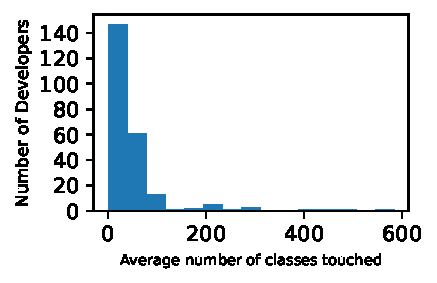
\includegraphics[width=\textwidth]{sections/results/graph/normality_and_homoscedasticity_graph_transient_moderate_10_classes_sample_sustained.classes.touched.commits.pdf}
    \caption{Sustained ($\mu$: 50.94, median:29, mode:13, std:73.73 and max:584)}
    \label{figure.sections/results/graph/normality_and_homoscedasticity_graph_transient_moderate_10_classes_sample_sustained.classes.touched.commits.pdf}
  \end{subfigure}
\caption{Classes for ten commits for  sample A category versus sample B category } 
\end{figure}
\clearpage 
\begin{figure}
  \centering 
\end{figure}
\clearpage 
\begin{figure}
  \centering 
\vspace{3mm}
  \begin{subfigure}[b]{0.45\textwidth}
    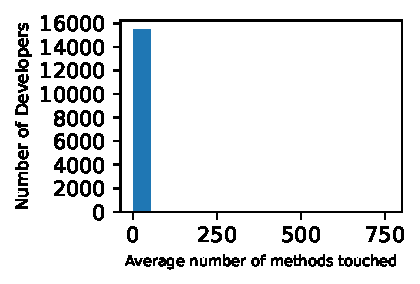
\includegraphics[width=\textwidth]{sections/results/graph/normality_and_homoscedasticity_graph_transient_moderate_1_methods_founder_transient.methods.touched.commits.pdf}
    \caption{Transient ($\mu$: 1.47, median:1.0, mode:1, std:9.29 and max:763)}
    \label{figure.sections/results/graph/normality_and_homoscedasticity_graph_transient_moderate_1_methods_founder_transient.methods.touched.commits.pdf}
  \end{subfigure}
  \begin{subfigure}[b]{0.45\textwidth}
    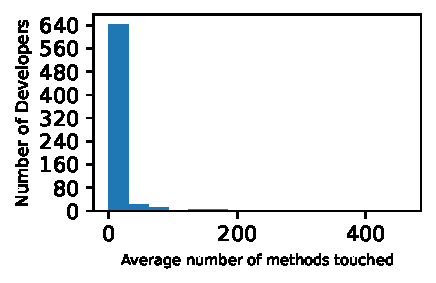
\includegraphics[width=\textwidth]{sections/results/graph/normality_and_homoscedasticity_graph_transient_moderate_1_methods_sample_moderate.methods.touched.commits.pdf}
    \caption{Moderate ($\mu$: 8.9, median:1, mode:1, std:33.8 and max:463)}
    \label{figure.sections/results/graph/normality_and_homoscedasticity_graph_transient_moderate_1_methods_sample_moderate.methods.touched.commits.pdf}
  \end{subfigure}
\vspace{3mm}
  \begin{subfigure}[b]{0.45\textwidth}
    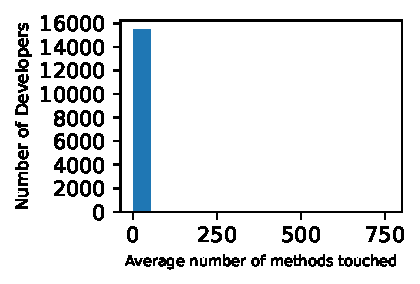
\includegraphics[width=\textwidth]{sections/results/graph/normality_and_homoscedasticity_graph_transient_moderate_1_methods_founder_transient.methods.touched.commits.pdf}
    \caption{Transient ($\mu$: 1.47, median:1.0, mode:1, std:9.29 and max:763)}
    \label{figure.sections/results/graph/normality_and_homoscedasticity_graph_transient_moderate_1_methods_founder_transient.methods.touched.commits.pdf}
  \end{subfigure}
  \begin{subfigure}[b]{0.45\textwidth}
    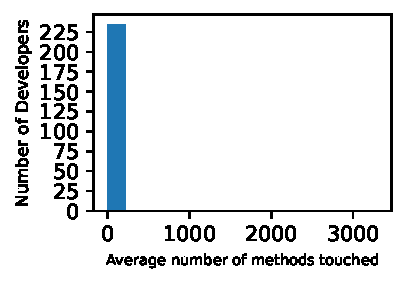
\includegraphics[width=\textwidth]{sections/results/graph/normality_and_homoscedasticity_graph_transient_moderate_1_methods_sample_sustained.methods.touched.commits.pdf}
    \caption{Sustained ($\mu$: 22.14, median:1, mode:1, std:218.06 and max:3301)}
    \label{figure.sections/results/graph/normality_and_homoscedasticity_graph_transient_moderate_1_methods_sample_sustained.methods.touched.commits.pdf}
  \end{subfigure}
\vspace{3mm}
  \begin{subfigure}[b]{0.45\textwidth}
    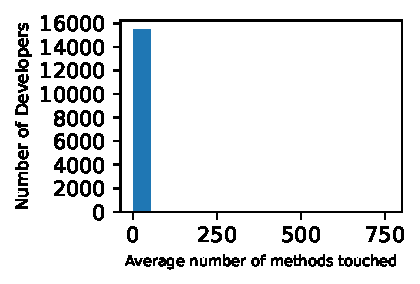
\includegraphics[width=\textwidth]{sections/results/graph/normality_and_homoscedasticity_graph_transient_moderate_1_methods_founder_transient.methods.touched.commits.pdf}
    \caption{Transient ($\mu$: 1.47, median:1.0, mode:1, std:9.29 and max:763)}
    \label{figure.sections/results/graph/normality_and_homoscedasticity_graph_transient_moderate_1_methods_founder_transient.methods.touched.commits.pdf}
  \end{subfigure}
  \begin{subfigure}[b]{0.45\textwidth}
    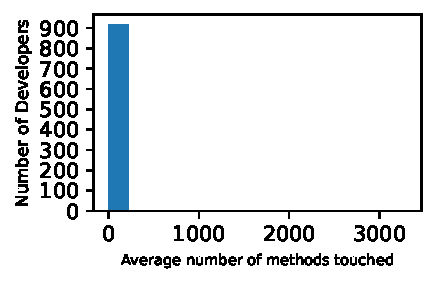
\includegraphics[width=\textwidth]{sections/results/graph/normality_and_homoscedasticity_graph_transient_moderate_1_methods_sample_moderate sustained.methods.touched.commits.pdf}
    \caption{Moderate sustained ($\mu$: 12.3, median:1.0, mode:1, std:114.2 and max:3301)}
    \label{figure.sections/results/graph/normality_and_homoscedasticity_graph_transient_moderate_1_methods_sample_moderate sustained.methods.touched.commits.pdf}
  \end{subfigure}
\vspace{3mm}
  \begin{subfigure}[b]{0.45\textwidth}
    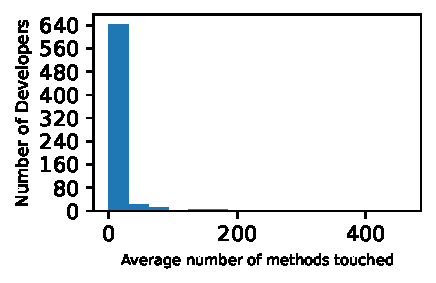
\includegraphics[width=\textwidth]{sections/results/graph/normality_and_homoscedasticity_graph_transient_moderate_1_methods_founder_moderate.methods.touched.commits.pdf}
    \caption{Moderate ($\mu$: 8.9, median:1, mode:1, std:33.8 and max:463)}
    \label{figure.sections/results/graph/normality_and_homoscedasticity_graph_transient_moderate_1_methods_founder_moderate.methods.touched.commits.pdf}
  \end{subfigure}
  \begin{subfigure}[b]{0.45\textwidth}
    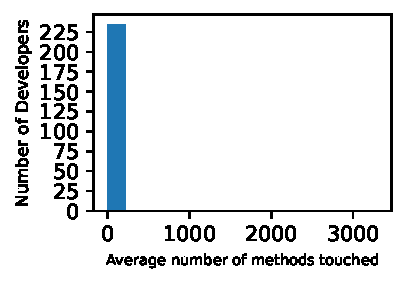
\includegraphics[width=\textwidth]{sections/results/graph/normality_and_homoscedasticity_graph_transient_moderate_1_methods_sample_sustained.methods.touched.commits.pdf}
    \caption{Sustained ($\mu$: 22.14, median:1, mode:1, std:218.06 and max:3301)}
    \label{figure.sections/results/graph/normality_and_homoscedasticity_graph_transient_moderate_1_methods_sample_sustained.methods.touched.commits.pdf}
  \end{subfigure}
\caption{Methods for one commits for  sample A category versus sample B category } 
\end{figure}
\clearpage 
\begin{figure}
  \centering 
\vspace{3mm}
  \begin{subfigure}[b]{0.45\textwidth}
    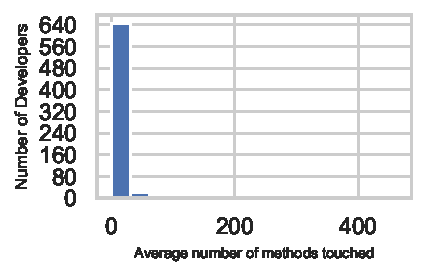
\includegraphics[width=\textwidth]{sections/results/graph/normality_and_homoscedasticity_graph_transient_moderate_2_methods_founder_moderate.methods.touched.commits.pdf}
    \caption{Moderate ($\mu$: 31.96, median:6, mode:1, std:84.15 and max:846)}
    \label{figure.sections/results/graph/normality_and_homoscedasticity_graph_transient_moderate_2_methods_founder_moderate.methods.touched.commits.pdf}
  \end{subfigure}
  \begin{subfigure}[b]{0.45\textwidth}
    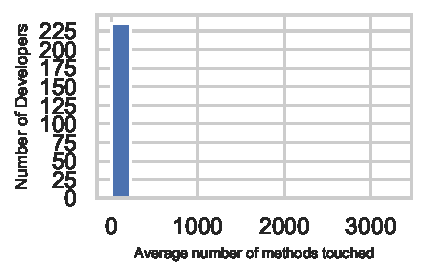
\includegraphics[width=\textwidth]{sections/results/graph/normality_and_homoscedasticity_graph_transient_moderate_2_methods_sample_sustained.methods.touched.commits.pdf}
    \caption{Sustained ($\mu$: 34.81, median:6, mode:1, std:164.27 and max:2022)}
    \label{figure.sections/results/graph/normality_and_homoscedasticity_graph_transient_moderate_2_methods_sample_sustained.methods.touched.commits.pdf}
  \end{subfigure}
\caption{Methods for two commits for  sample A category versus sample B category } 
\end{figure}
\clearpage 
\begin{figure}
  \centering 
\vspace{3mm}
  \begin{subfigure}[b]{0.45\textwidth}
    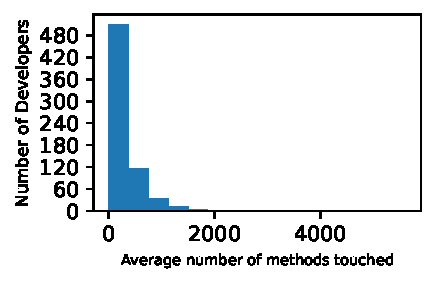
\includegraphics[width=\textwidth]{sections/results/graph/normality_and_homoscedasticity_graph_transient_moderate_5_methods_founder_moderate.methods.touched.commits.pdf}
    \caption{Moderate ($\mu$: 87.06, median:42, mode:10, std:180.93 and max:2970)}
    \label{figure.sections/results/graph/normality_and_homoscedasticity_graph_transient_moderate_5_methods_founder_moderate.methods.touched.commits.pdf}
  \end{subfigure}
  \begin{subfigure}[b]{0.45\textwidth}
    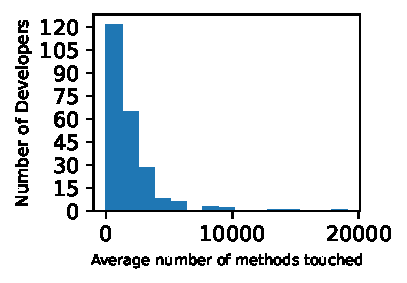
\includegraphics[width=\textwidth]{sections/results/graph/normality_and_homoscedasticity_graph_transient_moderate_5_methods_sample_sustained.methods.touched.commits.pdf}
    \caption{Sustained ($\mu$: 118.18, median:37, mode:15, std:337.13 and max:3559)}
    \label{figure.sections/results/graph/normality_and_homoscedasticity_graph_transient_moderate_5_methods_sample_sustained.methods.touched.commits.pdf}
  \end{subfigure}
\caption{Methods for five commits for  sample A category versus sample B category } 
\end{figure}
\clearpage 
\begin{figure}
  \centering 
\vspace{3mm}
  \begin{subfigure}[b]{0.45\textwidth}
    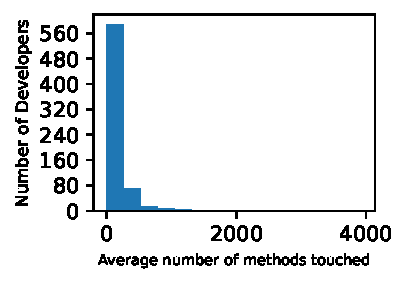
\includegraphics[width=\textwidth]{sections/results/graph/normality_and_homoscedasticity_graph_transient_moderate_10_methods_founder_moderate.methods.touched.commits.pdf}
    \caption{Moderate ($\mu$: 153.35, median:91.0, mode:18, std:245.1 and max:3940)}
    \label{figure.sections/results/graph/normality_and_homoscedasticity_graph_transient_moderate_10_methods_founder_moderate.methods.touched.commits.pdf}
  \end{subfigure}
  \begin{subfigure}[b]{0.45\textwidth}
    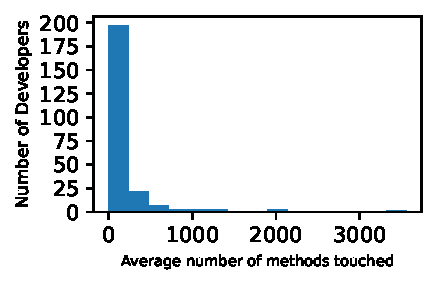
\includegraphics[width=\textwidth]{sections/results/graph/normality_and_homoscedasticity_graph_transient_moderate_10_methods_sample_sustained.methods.touched.commits.pdf}
    \caption{Sustained ($\mu$: 191.16, median:92, mode:18, std:359.45 and max:3561)}
    \label{figure.sections/results/graph/normality_and_homoscedasticity_graph_transient_moderate_10_methods_sample_sustained.methods.touched.commits.pdf}
  \end{subfigure}
\caption{Methods for ten commits for  sample A category versus sample B category } 
\end{figure}
\clearpage 
\begin{figure}
  \centering 
\end{figure}
\clearpage 
